% ============================================================
% 深圳大学实验报告 — Project 2 Classifier Visualization
% 基于 Experiment-Report-Template-SZU (Chao Fan, Kewei Ou)
% 编译方式：Overleaf 中选择 XeLaTeX
% ============================================================
\documentclass[a4paper,11pt]{article}

% ---------- 中文与字体 ----------
\usepackage{fontspec}
\usepackage{xeCJK}
\setCJKmainfont{Noto Serif CJK SC}
\usepackage{xcolor}

% ---------- 页面与常用宏包 ----------
\usepackage{geometry}
\geometry{left=0.85in, right=0.85in, top=0.8in, bottom=0.8in}
\usepackage{graphicx}
\usepackage{float}
\usepackage{subcaption}
\usepackage{longtable}
\usepackage{amsmath}
\usepackage{hyperref}
\hypersetup{colorlinks=true, linkcolor=black, urlcolor=blue}

% ---------- 代码红色高亮（满足 "Highlight Your Code in RED"） ----------
\usepackage{listings}
\lstset{
  basicstyle=\ttfamily\footnotesize\color{red},
  keywordstyle=\color{red},
  commentstyle=\color{red},
  stringstyle=\color{red},
  numbers=none,
  frame=single,
  framerule=0.4pt,
  rulecolor=\color{gray},
  xleftmargin=6pt, xrightmargin=6pt,
  breaklines=true,
  showstringspaces=false
}

% ---------- TikZ 工作流插图 ----------
\usepackage{tikz}
\usetikzlibrary{calc, arrows.meta, positioning}
\tikzset{
  block/.style={draw=#1!70!black, fill=#1!12, rounded corners,
                minimum width=26mm, minimum height=11mm,
                align=center, font=\footnotesize},
  arrow/.style={-{Stealth[length=2.2mm]}, gray, thick}
}

\begin{document}

% ============================================================
% 封面
% ============================================================
\begin{titlepage}
\centering
\vspace*{2cm}
\Huge{\textbf{深 \ 圳 \ 大 \ 学 \ 实 \ 验 \ 报 \ 告}}\\[1.5cm]
{\Large\textbf{课程名称}\quad\underline{\makebox[8cm][c]{Python程序设计}}}\\[0.5cm]
{\Large \noindent\makebox[3.2cm][l]{\textbf{项目名称}} \underline{\makebox[8cm][c]{分类器可视化}}}\\[0.5cm]
{\Large \noindent\makebox[3.2cm][l]{\textbf{学 \quad \quad 院}} \underline{\makebox[8cm][c]{人工智能学院}}}\\[0.5cm]
{\Large \noindent\makebox[3.2cm][l]{\textbf{专 \quad \quad 业}} \underline{\makebox[8cm][c]{人工智能}}}\\[0.5cm]
{\Large \noindent\makebox[3.2cm][l]{\textbf{指导教师}} \underline{\makebox[8cm][c]{舒婷}}}\\[0.5cm]
{\Large \noindent\makebox[3.2cm][l]{\textbf{报 \quad 告 \quad 人}} \underline{\makebox[3cm][c]{郑贺元}} \hspace{0.5cm} \textbf{学号} \underline{\makebox[3.6cm][c]{2025681028}}}\\[0.5cm]
{\Large \noindent\makebox[3.2cm][l]{\textbf{实验时间}} \underline{\makebox[8cm][c]{2026年11月末}}}\\[0.5cm]
{\Large \noindent\makebox[3.2cm][l]{\textbf{提交时间}} \underline{\makebox[8cm][c]{2026年11月末}}}\\[1.2cm]
{\large 代码仓库：\url{https://github.com/2058226971/project2-visualization}}
\vfill
\Large{\textbf{教务处制}}
\end{titlepage}
\newpage

% ============================================================
% 正文（控制在 5 页以内，不含封面）
% ============================================================

\section{实验目标 (Objectives)}
本实验的目标不是训练新模型，而是\textbf{把已训练分类器``在想什么''画出来}。我们在 Iris 数据集上完成四类可视化：比较两种二特征分类器的决策区域与概率图（任务 1）；画出二分类模型在三维特征空间中的 $P(\text{virginica})=0.5$ 决策平面（任务 2）；用彩色探针展示该概率在三维空间中的分布（任务 3）；最后做一个有解释的扩展——回放保存的训练状态，展示决策区域如何随训练推进而移动（任务 4）。所有绘图函数集中在 \texttt{tasks.py}，数据加载与模型拟合由给定的 \texttt{main.py} 完成，二者分离使每张图都可由相同输入复现。

\section{方案概览 (Overview)}
实验流程如图~\ref{fig:flow}：给定数据经标准化后同时送入两个模型；二维部分在花瓣长 $x_3$、花瓣宽 $x_4$ 上比较逻辑回归与随机森林，并用 $105$ 条训练、$45$ 条验证的分层划分（\texttt{random\_state=42}）评估；三维部分用全部 $100$ 朵非 setosa 花、在原始厘米单位下拟合二分类逻辑回归。三维与二维是两次不同的实验，报告中分别说明。

\begin{figure}[H]
\centering
\begin{tikzpicture}[node distance=5mm]
\node[block=blue] (data) {Iris 数据\\$x_3,x_4$ (cm)};
\node[block=green, right=of data, xshift=6mm] (model) {拟合模型\\LogReg / Forest};
\node[block=orange, right=of model, xshift=10mm] (grid) {探针网格\\$120\times160$ / 3D};
\node[block=blue, below=of data, yshift=-2mm] (t1) {任务1：2D\\区域 + 概率};
\node[block=green, below=of model, yshift=-2mm] (t2) {任务2/3：3D\\平面 + 概率};
\node[block=orange, below=of grid, yshift=-2mm] (t4) {任务4：扩展\\状态回放};
\draw[arrow] (data) -- (model);
\draw[arrow] (model) -- (grid);
\draw[arrow] (data) -- (t1);
\draw[arrow] (model) -- (t2);
\draw[arrow] (grid) -- (t4);
\end{tikzpicture}
\caption{实验工作流：数据、模型与四个可视化任务的关系}
\label{fig:flow}
\end{figure}

\section{实现细节 (Implementations)}
四个核心函数只负责绘图，不做拟合。关键实现如下（代码以红色高亮）。

\paragraph{任务 1：决策区域与概率图。}
用 \texttt{contourf} 在探针网格上填充预测类别，再把真实花朵以散点叠加；背景是模型的``答案''，点是``标准答案''，颜色不一致处即错分。概率图对每个物种画一个面板，三个面板共用固定的 $0$--$1$ 色标和相同等值线级别：
\begin{lstlisting}
ax.contourf(xx, yy, region, levels=[-0.5,0.5,1.5,2.5],
            cmap=REGION_CMAP, alpha=0.95)
ax.scatter(X[:,0], X[:,1], c=y, cmap=POINT_CMAP,
           vmin=0, vmax=2, edgecolors="white")
for k, ax in enumerate(axes):
    im = ax.contourf(xx, yy, probabilities[...,k],
                     levels=PROB_LEVELS, cmap=PROB_CMAPS[k],
                     vmin=0.0, vmax=1.0)
    fig.colorbar(im, ax=ax)
\end{lstlisting}

\paragraph{任务 2：三维决策平面。}
逻辑回归的对数几率是线性的：$s=w_2x_2+w_3x_3+w_4x_4+b$，$P(\text{virginica})=\sigma(s)$。$P=0.5$ 恰在 $s=0$，解出 $x_4$ 即得平面，模型在原始厘米单位下拟合，无需标准化：
\begin{lstlisting}
w2, w3, w4 = model.coef_[0]
b = model.intercept_[0]
x4 = -(w2*x2_grid + w3*x3_grid + b) / w4
ax.plot_surface(x2_grid, x3_grid, x4,
                color="#9AA0A6", alpha=0.45)
\end{lstlisting}

\paragraph{任务 3：三维概率探针。}
在特征空间均匀撒 $14^3=2744$ 个探针，一次性查询概率。模型 \texttt{classes\_=[1,2]}，virginica 是\textbf{第 1 列}（任务 1 三分类时是第 2 列，勿混淆），按类值定位可避免错位：
\begin{lstlisting}
p = model.predict_proba(probe)
q = p[:, list(model.classes_).index(2)]
ax.scatter(probe[:,0], probe[:,1], probe[:,2],
           c=q, cmap="plasma", vmin=0, vmax=1)
\end{lstlisting}

\paragraph{任务 4：保存状态回放（扩展）。}
读取 \texttt{learning\_states.npz} 中 301 组 $(W,b)$，在同一标准化探针网格上重画。参数变化、输入不变，因此能干净地展示``学习''本身：
\begin{lstlisting}
W, b = weights[epoch], biases[epoch]
logits = grid_std @ W + b
labels = logits.argmax(axis=1).reshape(shape)
# 用与任务1相同的 draw_frame 绘制每帧
\end{lstlisting}

\section{实验结果 (Results)}
\subsection{两种分类器对比（任务 1）}
图~\ref{fig:regions} 显示两者在同一坐标轴、同一验证集上的决策区域。逻辑回归的边界是直线（线性模型），随机森林的边界呈锯齿状（由轴平行的分裂拼成）。在 $45$ 朵留一验证花上，逻辑回归正确 $41$ 朵（$91.1\%$），随机森林正确 $43$ 朵（$95.6\%$）。两种颜色冲突的区域主要集中在 versicolor 与 virginica 的交界处——这是数据集本身重叠的部分，也是主要错误来源。

\begin{figure}[H]
\centering
\begin{subfigure}[b]{0.46\linewidth}
\centering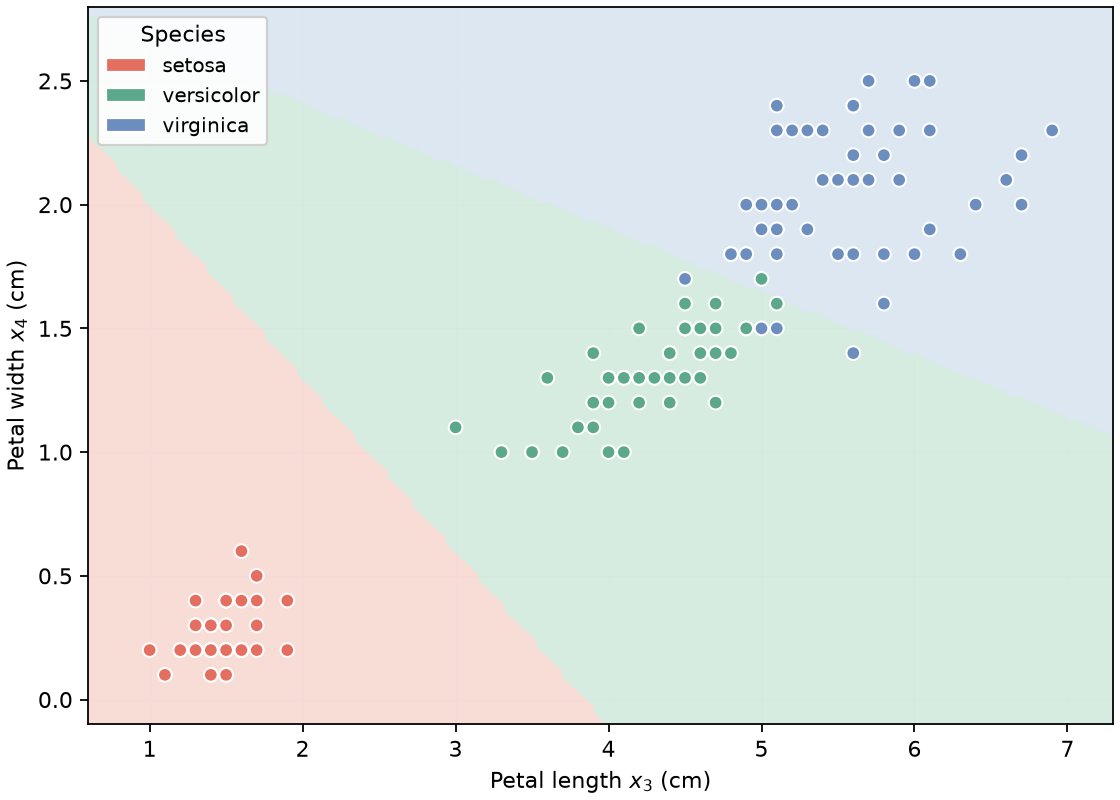
\includegraphics[width=\linewidth]{figs/logistic_regions.png}
\caption{逻辑回归：线性边界}
\end{subfigure}\hfill
\begin{subfigure}[b]{0.46\linewidth}
\centering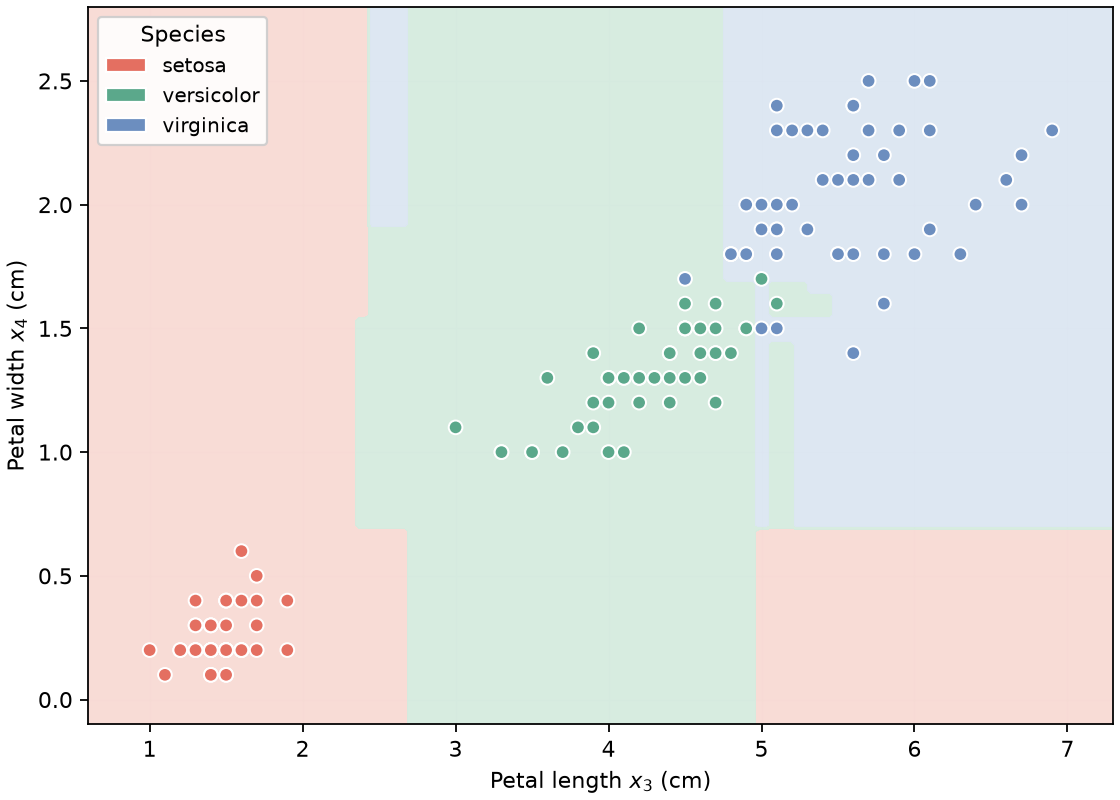
\includegraphics[width=\linewidth]{figs/forest_regions.png}
\caption{随机森林：锯齿状边界}
\end{subfigure}
\caption{任务 1：决策区域（横轴花瓣长 $x_3$/cm，纵轴花瓣宽 $x_4$/cm；珊瑚=setosa，绿=versicolor，蓝=virginica）}
\label{fig:regions}
\end{figure}

图~\ref{fig:prob} 给出逻辑回归三个物种的概率面板。每个面板色标固定 $0$--$1$：$P(\text{setosa})$ 在左下角趋近 $1$，$P(\text{virginica})$ 在右上角趋近 $1$，而 $P(\text{versicolor})$ 在中间形成一条带状高值区，正是它被另外两类夹住的直接体现。森林的概率图结构相似但过渡更陡。

\begin{figure}[H]
\centering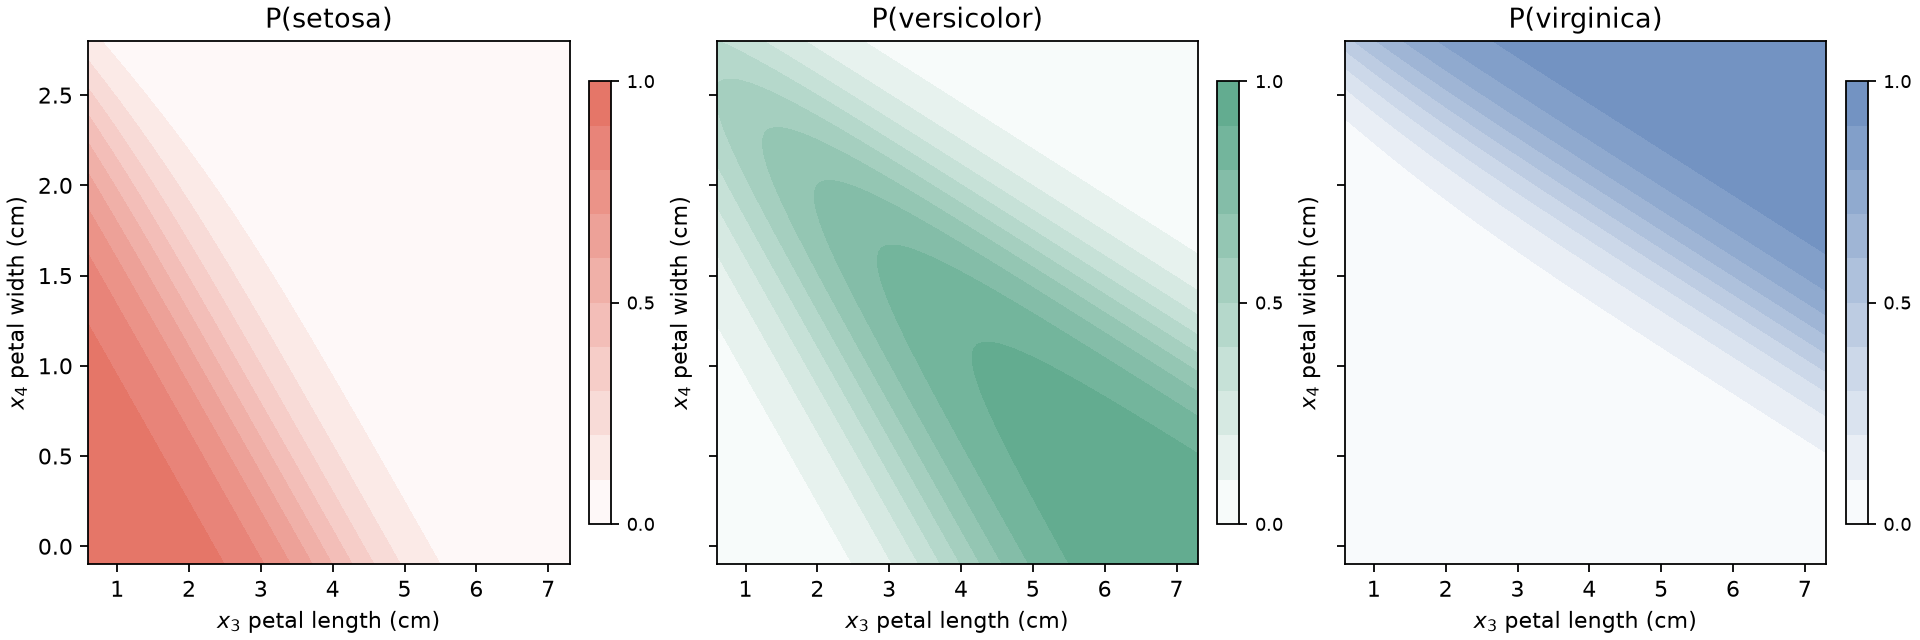
\includegraphics[width=0.95\linewidth]{figs/logistic_probabilities.png}
\caption{任务 1：逻辑回归的逐类概率图，三个面板共用 $0$--$1$ 色标}
\label{fig:prob}
\end{figure}

\subsection{三维边界与概率（任务 2、3）}
图~\ref{fig:plane} 中灰色平面即 $P(\text{virginica})=0.5$ 的分界面，三个坐标轴为 $x_2$（萼片宽）、$x_3$（花瓣长）、$x_4$（花瓣宽），单位均为厘米。由 $s=0$ 可知该面是线性的：固定 $x_2,x_3$ 时可解出唯一的 $x_4$ 使两类打平；点位于平面上方时 $s>0$，更可能是 virginica，下方则更可能是 versicolor。

\begin{figure}[H]
\centering
\begin{subfigure}[b]{0.46\linewidth}
\centering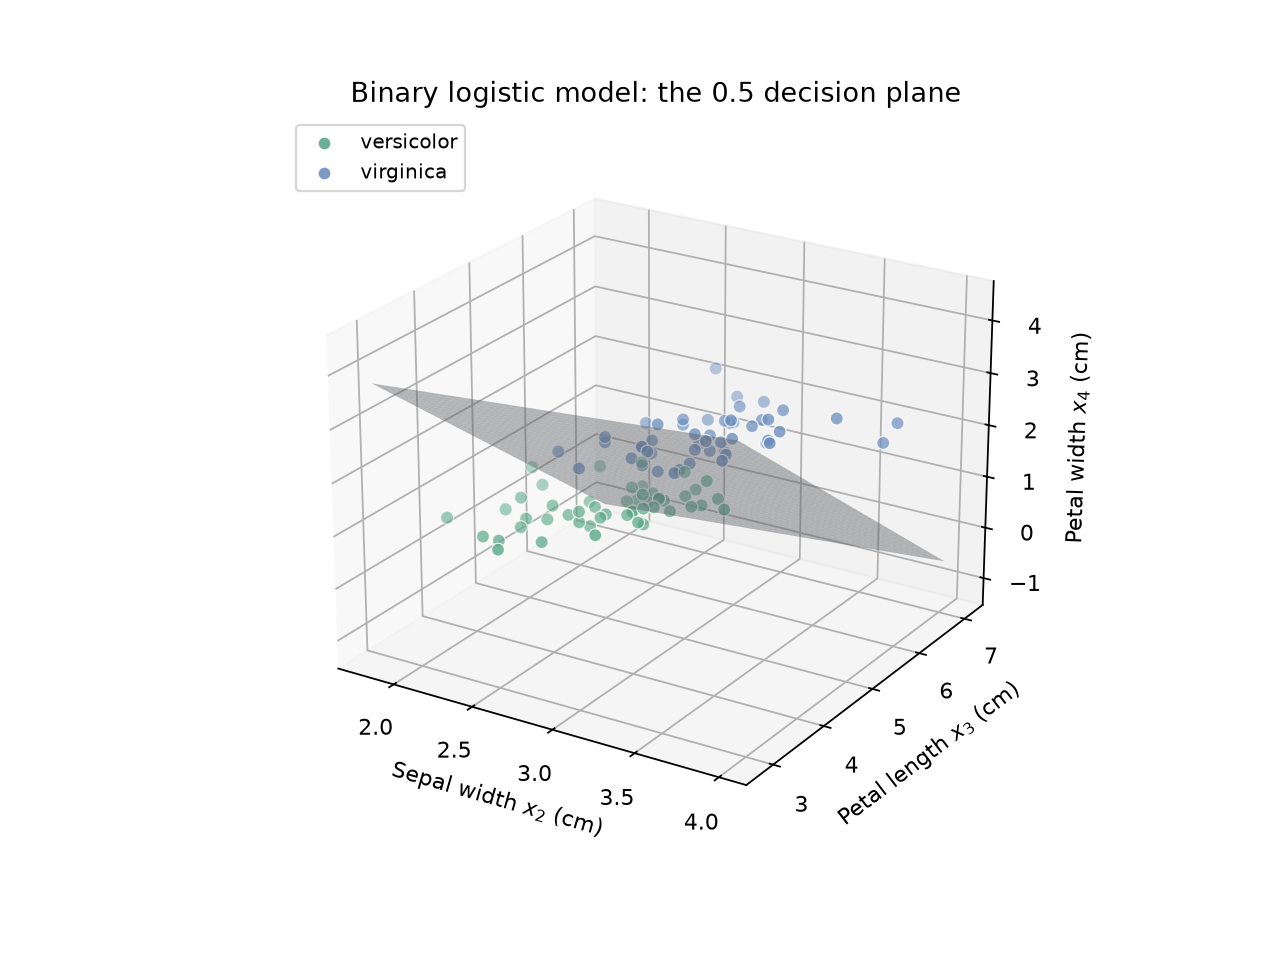
\includegraphics[width=\linewidth]{figs/boundary_3d.png}
\caption{0.5 决策平面与观测点}
\end{subfigure}\hfill
\begin{subfigure}[b]{0.46\linewidth}
\centering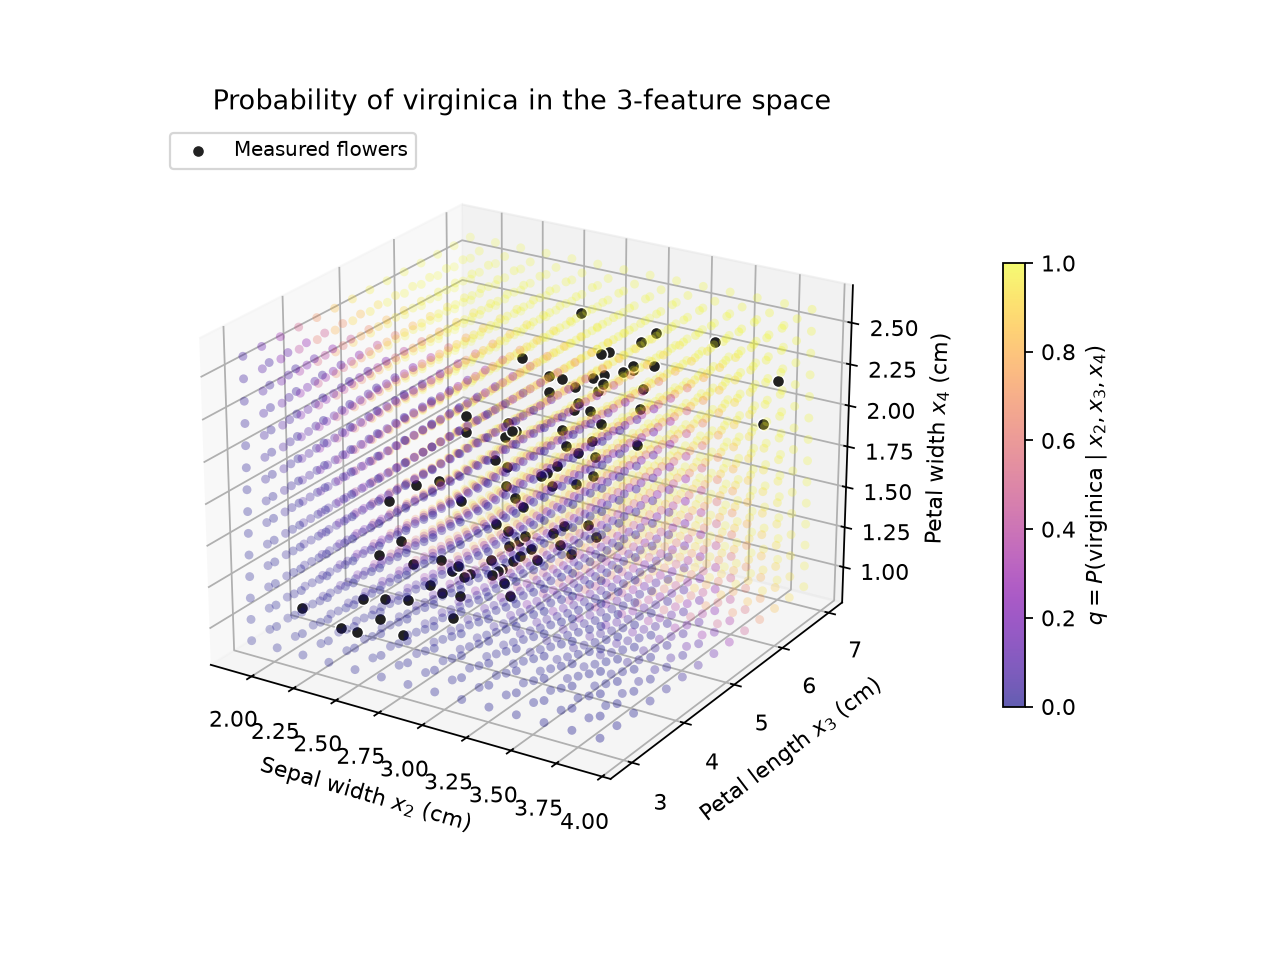
\includegraphics[width=\linewidth]{figs/probability_3d.png}
\caption{彩色探针显示 $q=P(\text{virginica})$}
\end{subfigure}
\caption{任务 2、3：同一二分类模型的三维几何（色标固定 $0$--$1$，紫=低概率，黄=高概率）}
\label{fig:plane}
\end{figure}

图~\ref{fig:plane}(b) 用颜色把概率铺满三维空间：靠近平面处颜色约为 $0.5$，远离时过渡到紫色（接近 versicolor）或黄色（接近 virginica）。它与图~\ref{fig:plane}(a) 是同一模型的两种视角——一个是``边界在哪''，一个是``置信度多高''。

\subsection{扩展：训练过程回放（任务 4）}
图~\ref{fig:replay} 是本次扩展的产出。上排三幅小图分别是第 $0$、$15$、$300$ 个保存状态的决策区域：初始时区域几乎随机；到 $15$ 轮已大致分开 setosa；第 $300$ 轮时三块区域清晰稳定。右下曲线给出训练与验证准确率：验证准确率由 $26.7\%$ 升至 $68.9\%$（第 $15$ 轮）再到 $91.1\%$（第 $300$ 轮）。此外还输出了 $31$ 帧动画 \texttt{learning\_replay.gif}，可连续观察边界移动。这说明模型确实是通过逐步调整 $(W,b)$ 把决策面搬到正确位置，而不是一开始就``知道''答案。

\begin{figure}[H]
\centering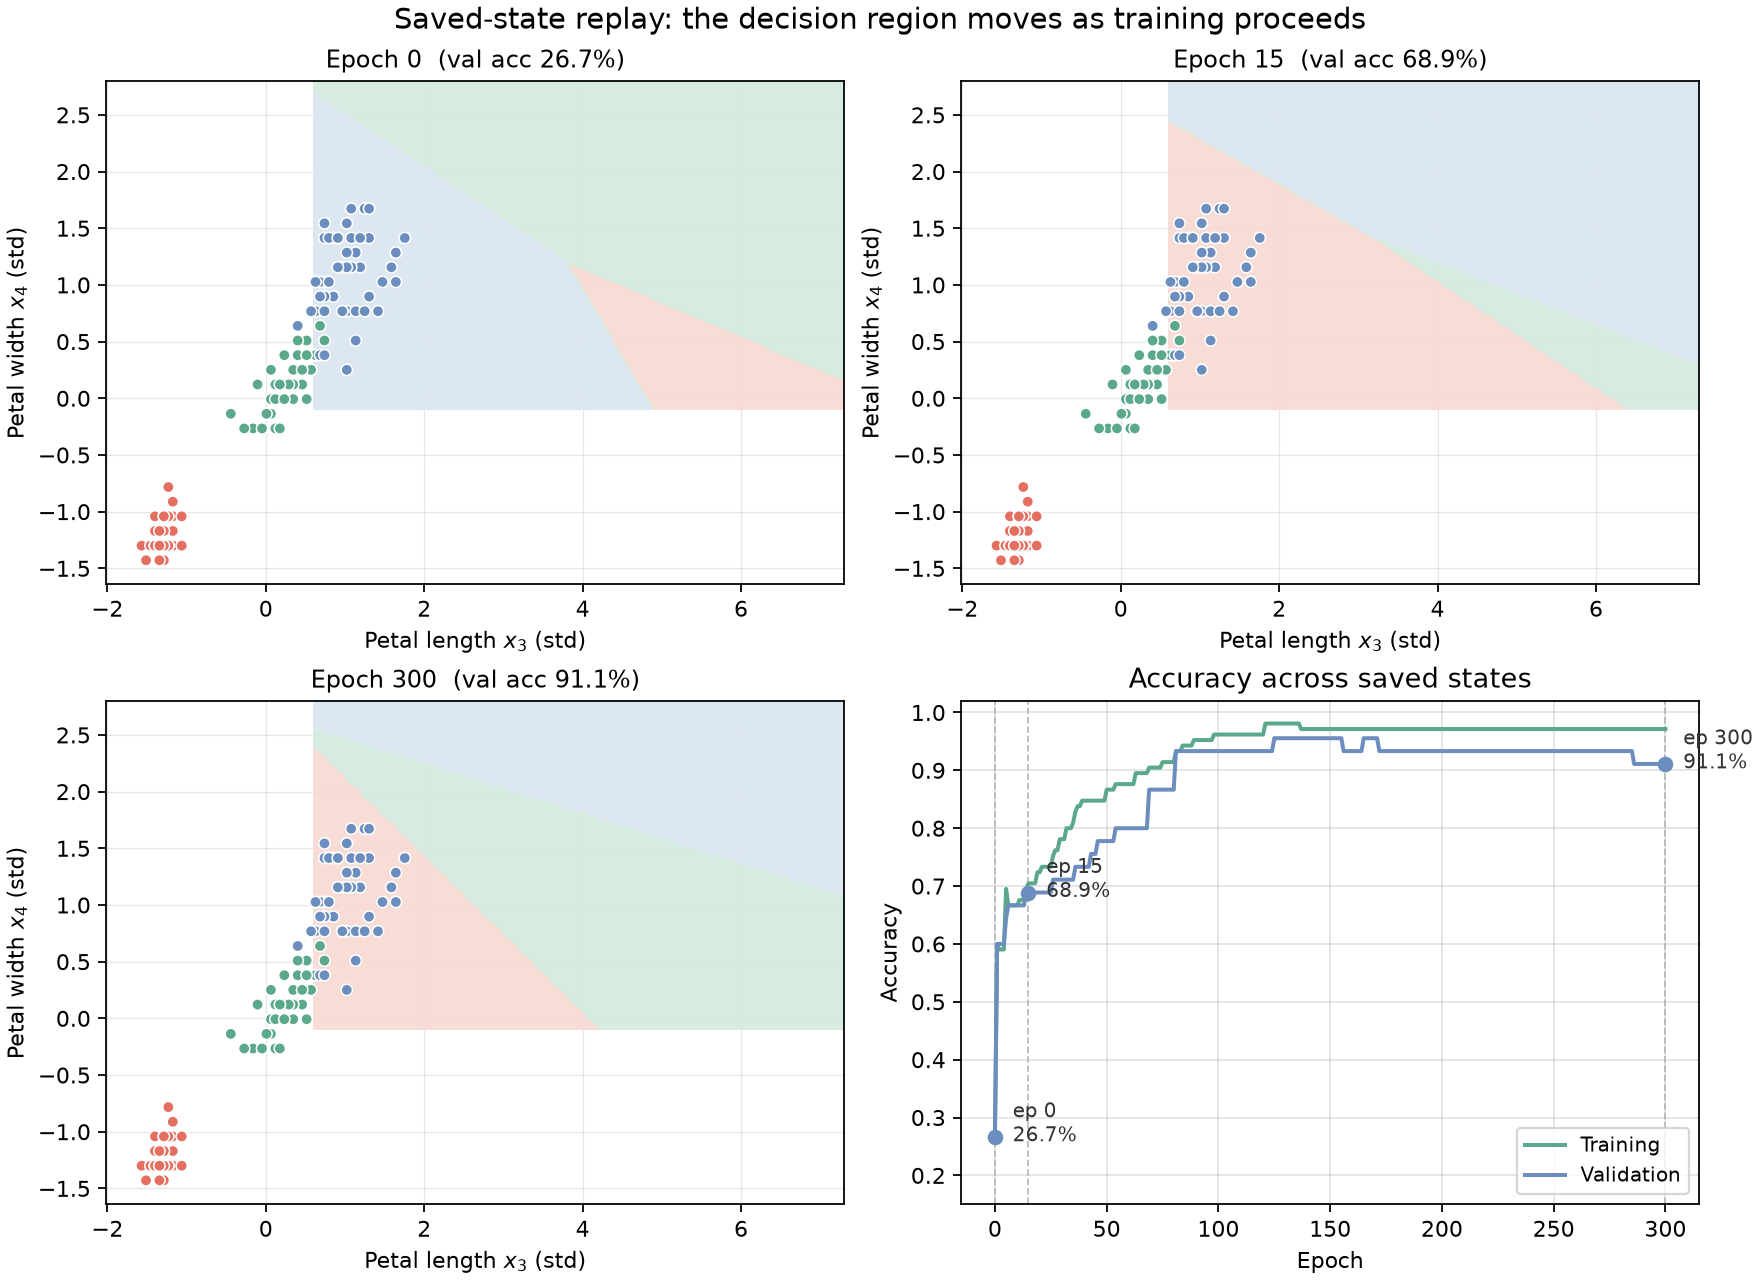
\includegraphics[width=0.92\linewidth]{figs/learning_replay.png}
\caption{任务 4：保存状态回放——上排为三个epoch的决策区域，右下为训练/验证准确率曲线}
\label{fig:replay}
\end{figure}

\section{讨论与结论 (Discussion)}
\textbf{个人贡献：}四个绘图函数、扩展脚本 \texttt{extension.py}、全部图表的排版与解释、README 与本报告由本人完成；数据加载与模型拟合沿用课程给定的 \texttt{main.py}。所有代码带充分注释，便于复现。

\textbf{关键教训：}一是类别顺序必须与 \texttt{classes\_} 对齐，三分类时 virginica 在概率第 $2$ 列，二分类时在第 $1$ 列，直接写死列号会默默画错图；二是概率色标必须显式固定 $0$--$1$，否则不同面板的色标被数据范围拉伸后无法横向比较；三是二维对比用 held-out $45$ 朵、三维模型用全部 $100$ 朵训练，两者评估口径不同，不能混为一谈。

\textbf{结论：}随机森林在验证集上略优于逻辑回归，但代价是边界不平滑、可解释性弱；线性模型的平面与概率梯度在三维中给出清晰几何图像。保存状态回放把抽象的``训练''变成了可见的边界移动，是本次扩展最有价值的可视化。完整代码与动画见 \url{https://github.com/2058226971/project2-visualization}。

% ============================================================
% 批阅与成绩评定页（模板自带）
% ============================================================
\newpage
\begin{tikzpicture}[remember picture, overlay]
\draw[thick] ($(current page.north west)+(2cm,-3cm)$) rectangle ($(current page.south east)+(-2cm,3.5cm)$);
\end{tikzpicture}
\vspace{1cm}
\noindent \textbf{指导教师批阅意见：}
\vspace{6cm}
\hfill
\vspace{1cm}
\noindent \textbf{成绩评定：}
\vspace{2cm}
\hfill
\vspace{1cm}
\noindent \hfill \textbf{指导教师签字：}\quad\quad\quad\quad\quad\\[0.5cm]
\hfill \textbf{年}\quad\quad \textbf{月}\quad\quad \textbf{日}\quad
\vspace{1cm}
\noindent \textbf{备注：}
\begin{tikzpicture}[remember picture, overlay]
\node[ anchor=north west, inner sep=0pt, text width=\dimexpr\paperwidth-4cm\relax ]
at ($(current page.south west)+(2cm,3.1cm)$) {
\begin{minipage}{\dimexpr\paperwidth-4cm\relax}
\small
\noindent \textbf{注：}\;1、报告内的项目或内容设置，可根据实际情况加以调整和补充。\\[0.2cm]
\phantom{\textbf{注：}\;}2、教师批改学生实验报告时间应在学生提交实验报告时间后 10 日内。
\end{minipage} };
\end{tikzpicture}

\end{document}
